\documentclass[10pt,letterpaper]{article}

\usepackage{cogsci}
\usepackage{pslatex}
\usepackage{apacite}
\usepackage{graphicx}
\usepackage{caption}
%\usepackage{subcaption}
\usepackage{subfigure}
\graphicspath{{figures/}}
  
\begin{document}

\title{Some arguments are probably valid}
 
\author{{\large \bf M. H. Tessler, Noah D. Goodman } \\
	\{mhtessler, ngoodman\}@stanford.edu \\
  Department of Psychology, Stanford University}

\maketitle


\begin{abstract}
This is not an abstract.\\
\textbf{Keywords:} 
Reasoning, probabilistic model
\end{abstract}

Syllogistic reasoning has been a topic of considerable interest in cognitive psychology for over one hundred years, and before that in philosophy, dating back to Aristotle. A syllogism is a two premise argument, which relates two terms by a middle term. The relation is a quantifier, and the quantifiers used in the classical syllogism are all, some, none, and not all. For example,

\begin{quotation}
All artists are bakers\\
Some bakers are chemists\\
\end{quotation}

is a syllogistic argument. There are 64 possible syllogism which one can derive by replacing the quantifiers with others from the allowable set and reordering the terms (All As are Bs --> All Bs are As). Most syllogisms have no valid conclusion, like the one presented above. 

People with no training in formal logic, and even some with training, find reasoning with syllogisms difficult. A recent meta-analysis showed that over the population, accuracy on producing valid conclusions ranges from 90 \% to 1\% \cite{khemlaniJL2012}. For syllogisms with no valid conclusion, accuracy ranges from 76\% to 12\%.

This evidence would seem to suggest that people are not reasoning using deductive mechanisms in the mind. Yet, many theories take deduction as a given and try to explain errors as a matter of noise in the system. We take a different path. We propose, as has been proposed before, that people are reasoning according to their {\emph everyday} mode of reasoning. {\emph Everyday} reasoning is understood as the type of reasoning that is refined for dealing with a world of uncertainty, a world in which you don't know how many people are in the hallway outside your door or whether or not the lion is going to start charging. This type of reasoning is most succinctly described in the language of probability theory. In this formalism, deduction emerges as that which is most probable.

%
%Theories of syllogistic reasoning have been  One possibility is {\emph{logical deduction}. When a theory takes deduction to be fundamental, the explanatory power of the theory derives from explaining errors in deductive inference. That is to say, these theories treat the variety of performance errors as the first-class explanandum.
%
%We take a different path. We propose, as has been proposed before, that people are reasoning according to their {\emph everyday} mode of reasoning. {\emph Everyday} reasoning is understood as the type of reasoning that is refined for dealing with a world of uncertainty, a world in which you don't know how many people are in the hallway outside your door or whether or not the lion is going to start charging. This type of reasoning is most succinctly described in the language of probability theory. 

In the rest of the paper, we review three theories of syllogistic reasoning -- Mental Models, Mental Logics and Probability Heuristics -- which we take to exemplify three quadrants of a two-dimensional theoretical space. We develop a computational level theory in the unexplored quadrant of the space, instantiated in a probabilistic model. We compare our model predictions with the predictions of the other theories as well to behavioral data from a recent meta-analysis. We explore the flexibility of the model to account for reasoning behavior in a study using the generalized quantifiers most and few. We conclude by discussing further predictions of the model and future directions.  

\section{Extant theories}

A recent meta-analysis carved the space of reasoning theories into three partitions: those based on model or diagrammatic reasoning, those based on formal logical rules, and those based on heuristics \cite{Khemlani2012}. We see the space differently. In one dimension, theories may be based on applying rules -- be they heuristic or logical -- or they are based on constructing concrete representations or models. In another dimension, theories may be considered fundamentally probabilistic or deterministic. 

\subsection{Mental Models}
 The Mental Models Theory (MMT) describes a psychological process by which people reason by constructing {\em iconic} mental representations or models, which represent the terms of a proposition as a collection of individuals. In syllogistic reasoning, a model is constructed for each premise, and premise models are consolidated so that the conclusion may be ``read off" the joint model. For example, a model for the premise  \emph{All artists are bakers} could be represented as the following situation.

\begin{tabular}{l l}
artist & baker\\
artist & baker\\
 & baker\\
\end{tabular}

This shows 2 individuals who are both artists and bakers, and one individual who is a baker but not an artist. Thus, each row is a representation of the properties of an individual. The authors emphasize the need to search for counter-examples to check for logical validity. Errors arise in this search process.

The MMT captures the intuition that people are able to reason about sets of things explicitly and with respect to context.  The a priori believability of propositions has been shown to have an important effect on reasoning \cite{Oakhill1989}. Mental models are flexible in that content can motivate one to carry on the search process longer. The search process allows for individual differences insofar as some individuals may test many models and some may test just one. At the same time, the theory is not well defined insofar as it does not specify how various models come into existence, only that various models can come into existence.

%Different quantifiers can be applied by reasoning over these mental models; indeed one just needs to ``read off" the model to see if a certain proposition is true. Thus, it has been proposed that mental models could account for usage of generalized quantifiers (e.g. most and few) in syllogistic reasoning, though this claim has not been substantiated by empirical work or a model.

\subsection{Mental Logics}

Rips (1994) proposed that people reason according to rules of \emph{natural deduction}. The theory of Mental Logics, instantiated in the PSYCOP model, posits individuals construct \emph{logical sentences} in a language of first-order predicate calculus which are linked when the ``individual recognizes [the link or inference] as intuitively sound". The model explains errors as a failure to recognize the applicability of a given formal rule, a failure to retrieve the rule, or a failure to carry out the necessary steps for that rule. People are especially prone to such errors when complex rules are needed so there is a predicted effect of rule complexity on difficulty. In this instance, the theory does not specify \emph{which} conclusions will be drawn fallaciously, only that some will. Mental Logics posits that people reason according to logical, deterministic rules. 

\subsection{Probability Heuristics}

Heuristic accounts be understood in a similar way: that people reason according to heuristic rules, which may be determined by probabilities. This the case with Chater and Oaksford's Probability Heuristic Model (PHM). Like our approach, the PHM is inspired by the notion that people are not fundamentally deductive reasoners, but instead are trying to gage degrees of plausibility for the conclusion. This amounts to computing the probability of a particular conclusion being true given that the premises are true. [equation] To accomplish this, the PHM relies on a number of {\em generation} and {\em test} heuristics which produce and quantify confidence in conclusions, and which they claim are justified by their computational level theory. The computational level theory includes a notion of informativeness, on which all their heuristics rely. We do not believe their heuristics are necessary for deriving a probabilistic model of reasoning, as we discuss below. Further, as is the case for theories based on formal rules, the very nature of their heuristics suggests reasoners are not engaging with the syllogisms at a semantic level. We also do not believe this to be the case. 


\section{The Conditional Semantics model}

The motivation for our model stems from two intuitions: (1) people are using \emph{everyday} reasoning in syllogistic reasoning tasks and (2) they do this by constructing situations \footnote{These situations are in no way different from mental models. We prefer the term situation so as to not confound the word model, which we take to refer to a computational model.} and reasoning over these situations. This formulation places the theory in the unexplored quadrant of the two-dimensional theoretical space described above: we consider reasoning over situations and situations to be constructed probabilistically. We use a naive binomial prior to sample situations. Each situation is composed of some number of objects, each with 1, 2 or 3 of the properties under discussion, exactly like in MMT. 

We draw on work in formal semantics by assuming that sentences are truth-functional operators. Thus, for a given situation, sentences are either true or false. By sampling over many situations, we construct a distribution over sentences, shown in Figure 1a.

For reasoning over syllogisms, the prior distribution is conditioned on the truth of the premise sentences. This is the distribution over sentences conditioned on the fact that the premises are true. In this way, we evaluate the $\Pr$(conclusion $\arrowvert$ premises). This is essentially a metric of the plausibility of the argument. In this formulation, $\Pr$(conclusion $\arrowvert$ premises) = 1 if and only if the syllogism is logically valid.

%
%To set this parameter, we follow Johnson-Laird's principle of parsimony, which states that situations are constructed to ``maximize the number of properties of each individual to try to keep the number of \emph{distinct sorts} of individuals to a minimum".
%
%, from which we accept only those consistent with the premises \footnote{We follow J-L's lead by imposing the additionasl constraint that the syllogistic terms refer to non-empty classes in the world. This is the existential presupposition.}.
%
%The basic model has two parameters, which both contribute to the concept of Expected Value: situation size and property rarity. We tested a number of situation sizes and found 6 to be the best. This is consistent with Johnson-Laird's principle of parsimony which states that models are constructed to ``maximize the number of properties of each individual to try to keep the number of \emph{distinct sorts} of individuals to a minimum". 
%
%The number of distinct sorts of individuals is highest for logically invalid syllogisms precisely because the problems are not fully constrained. In Johnson-Laird's examples of these types of models, the number of individuals is always 6. 
%
%Rarity refers to the probability that a particular object in a world has a property (or belongs to class). A principle of rarity is often assumed in line with the intuition that properties are relative rare \footnote{This article is an article and it's about reasoning, but it's not a cat, and it's not a car, nor an elephant nor the color red. In fact, there's a very large number of things which this article is not.}, and we assume a principle of rarity here. We tested a number of rarity factors and found that p=0.25 provided the best fit. This is also consistent with Chater \& Oaksford's rarity assumption. 

\subsection{Model predictions}

Our model assumes that properties are relatively rare of objects.  A principle of rarity is often assumed in line with the intuition that properties are relative rare \footnote{This article is an article and it's about reasoning, but it's not a cat, and it's not a car, nor an elephant nor the color red. In fact, there's a very large number of things which this article is not.}, and we assume a principle of rarity here. We tested a number of rarity factors and found that p=0.25 provided the best fit. This is also consistent with the Probability Heuristic's rarity assumption. 


\subsubsection{The Prior}
It might be the case that individuals are drawing conclusions simply from the prior probability of those conclusions being true. We show that this is not the case. From the prior, however, we can see that all conclusions are not equally likely. In particular, we observe an ordering which has previously been cited as an ordering of Informativity. The Probability Heuristics Model derives this ordering by positing categories as hyperspheres in a high-dimensional concept space \cite{Chater1999}. This ordering comes out of the Conditional Semantics Model with no further assumptions.

\subsubsection{Conditional Semantics}

The Conditional Semantics model conditions on the truth of the premises. The model generates situations in which the premises are true, and determines which conclusions are true in the variety of situations. In the limit, this converges to the $\Pr$(conclusion $\arrowvert$ premises). 

 Crucially, it doesn't match any of the syllogisms for which people like the all conclusion. One such syllogism is the canonical ``All/all" syllogism:

\begin{quote}
All Xs are Ys \\
All Ys are Zs \\
\end{quote}

This illustrates one of the issues with the conditional semantics model: it is too literal. The model computes the probability of the conclusion conditioned on the premises being true. For logically valid syllogistic conclusion, this probability is equal to 1. In particular, for any syllogism for which one of the universal quantifiers is valid (i.e. {\emph none} and {\emph all}), the particular quantifier (i.e. {\emph not all} and {\emph some}, respectively) will also be valid. Data from a number of experiments suggests that people do not treat {\emph all} and {\emph some} as equally correct or good conclusions. Instead, participants show a preference for conclusions the universal conclusions (all and none) when they are warranted. 

To address this we draw on recent advances in computational models of pragmatic reasoning. The rational speech-act theory addresses the problem of language understanding as that of a speaker trying to convey information about a world or situation that the speaker has observed \cite{Frank2012a}. The speaker draws on common-ground of communicative goals to maximize information content of a given utterance. In particular, choosing an utterance in proportion to the likelihood of a listener inferred the situations about which the speaker wishes to convey information. In turn, a listener considers situations in which the given utterance heard is not only true but would be chosen to disambiguate amongst multiple consistent situations. This results in canonical ``scalar implicature" wherein the literal meaning of ``{\em some} of the apples are red" is enriched to communicate ``{\em not all} of the apples are red".

We draw on this work by saying reasoners are not only choosing conclusions which are likely to be true but also which are informative. This makes the prediction that when given equally likely conclusions, reasoners will choose the one with the higher information content. Information content can be understood as an reciprocal function of the prior. Utterances or conclusions which are likely to be true a priori are preferred less than those which are less likely to be true. 

We operationalize this by using a variant of the nested-conditioning model of inference discussed in \cite{Goodman2013}. In the original model, the listener hears an utterance and tries to reconstruct the situation observed by the speaker. In our model, the reasoner chooses a conclusion consistent with the premises, while the listener hears the conclusion and tries to reconstruct the premises the reasoner was presented with. This is important as the reasoner does not observe a situation directly but rather constructs one consistent with the premises. 

\section{Results}

\subsection{Meta-analysis data}
To test our model, we used data from the meta-analysis presented with Probability Heuristics Model. These data were compiled from 5 studies on syllogistic reasoning, dating from 1978-1984. 

The data included percentage response of ``No Valid Conclusion". We consider the production of the ``No Valid Conclusion" an aspect of the algorithmic implementation and leave this for future work. In its most basic form the model produces responses corresponding to 1 of 4 quantifiers. The meta-analysis includes studies for which conclusion orderings were relaxed, such that participants could respond in either the A-C or the C-A ordering. Because of this, we allowed our model to do the same. Following the procedures of the meta-analysis, we collapsed responses across these two orderings to compare it to the data set.
\subsection{Model predictions}
For each model, we report the total number of syllogisms the model gets correct as well as the overall fit. A syllogism is deemed ``correct" if the model's maximum predicted response is the same as the most popular response in the meta-analysis data. This is a qualitative assessment of the fit. We compute correlations to assess the overall fit quantitatively. 

We first examined the prior to see if it alone accounted for human reasoning patterns. It did not. Since ``not all" is the most likely conclusion to be true, the prior gets only the syllogisms with a ``Not all" conclusion correct. For the meta-analysis data, this amounts to 29 out of the 64 syllogisms. The overall fit is also quite poor (r = .36). 

When we condition on the premises being true, the model matches people's maximum judgments on 37 of the 64 syllogisms. This includes all the syllogisms for which ``not all" is the maximum, as well as 8 syllogisms for which ``some" and ``none" are favored. The overall correlation is accordingly higher (r=0.62). However, among valid conclusions the correlation is terrible (r=-.20). This is a direct consequence of the model being logical and people not. Among valid conclusions to valid syllogisms, the model ranks them all equally high. 

By introducing pragmatics to the model, we are able to distinguish among equally ``plausible" conclusions. The model selects not only conclusions likely to be true, but conclusions which are informative to a hypothetical listener. The model now gets 44 out of 64 questions correct and has a correlation of r = 0.77. The difference is especially striking for the valid syllogisms, for which the correlation is now r = 0.82. 


%

\begin{figure*}[t!] %[htp]
\centering
  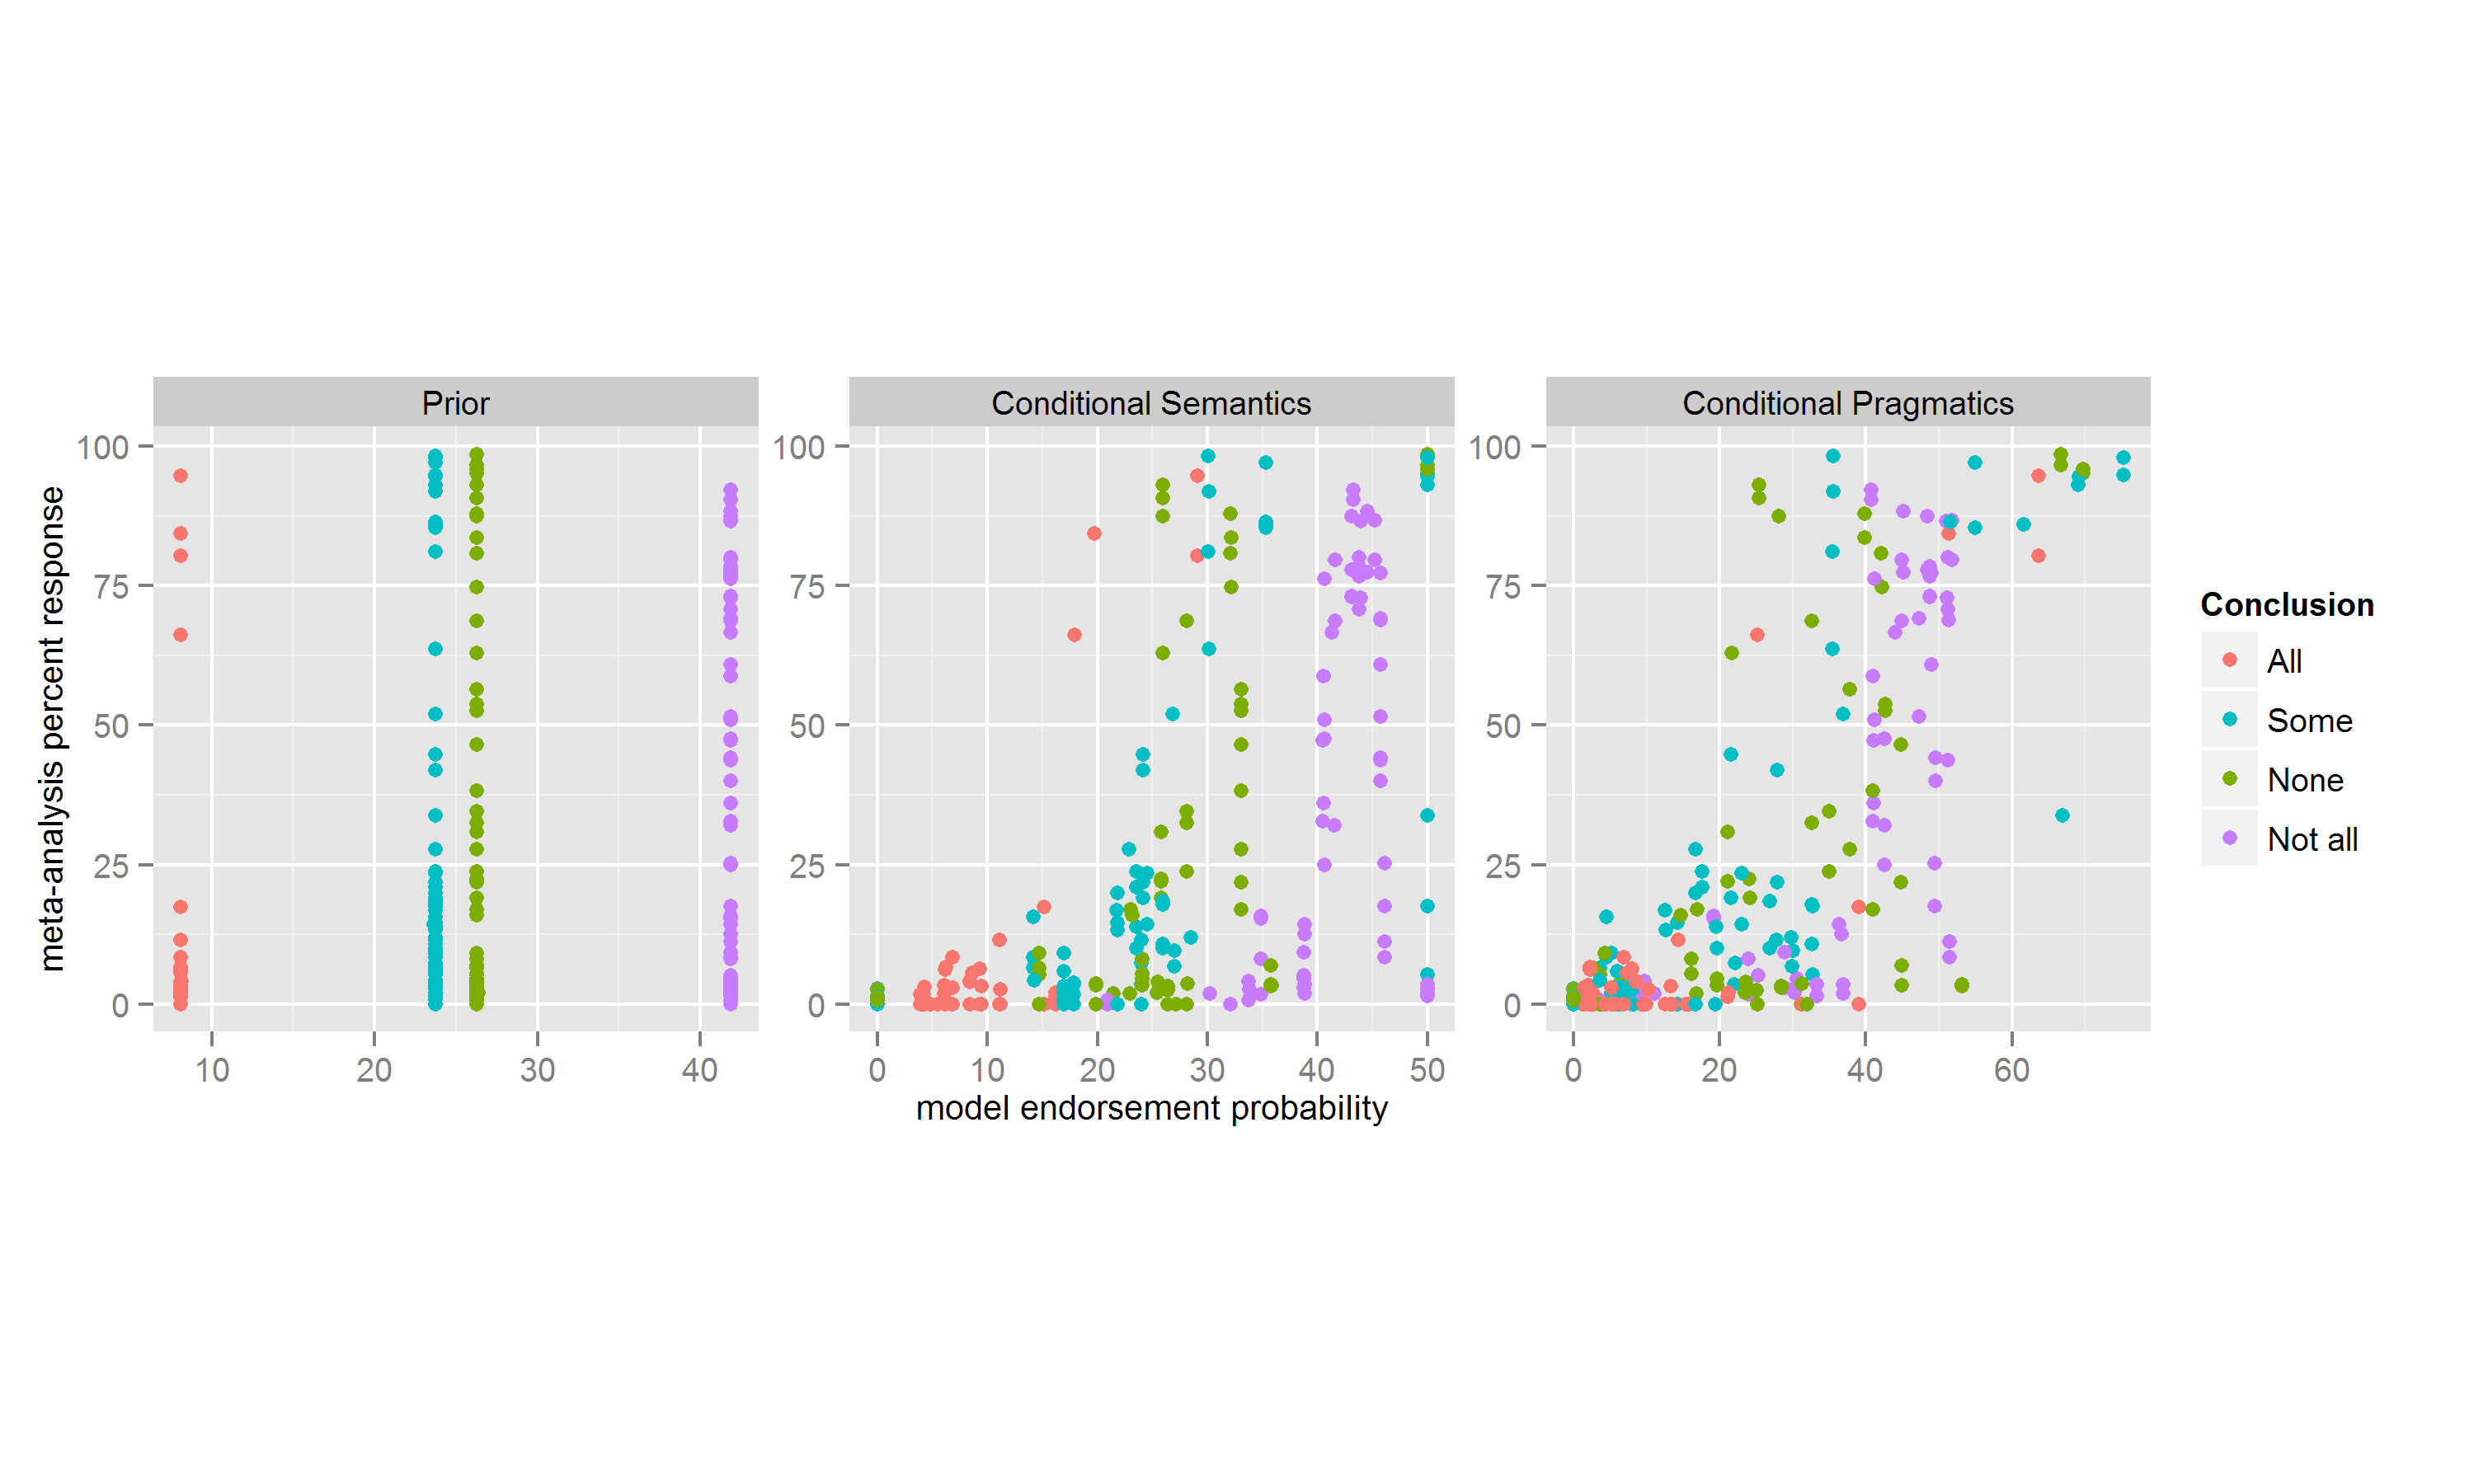
\includegraphics[width=\textwidth,height=10cm]{multiScatter_n6_0,25_alpha1}
  \caption{This is a tiger.}
\end{figure*}
%\end{figure*}
%\subfigure[prior]{ %
%	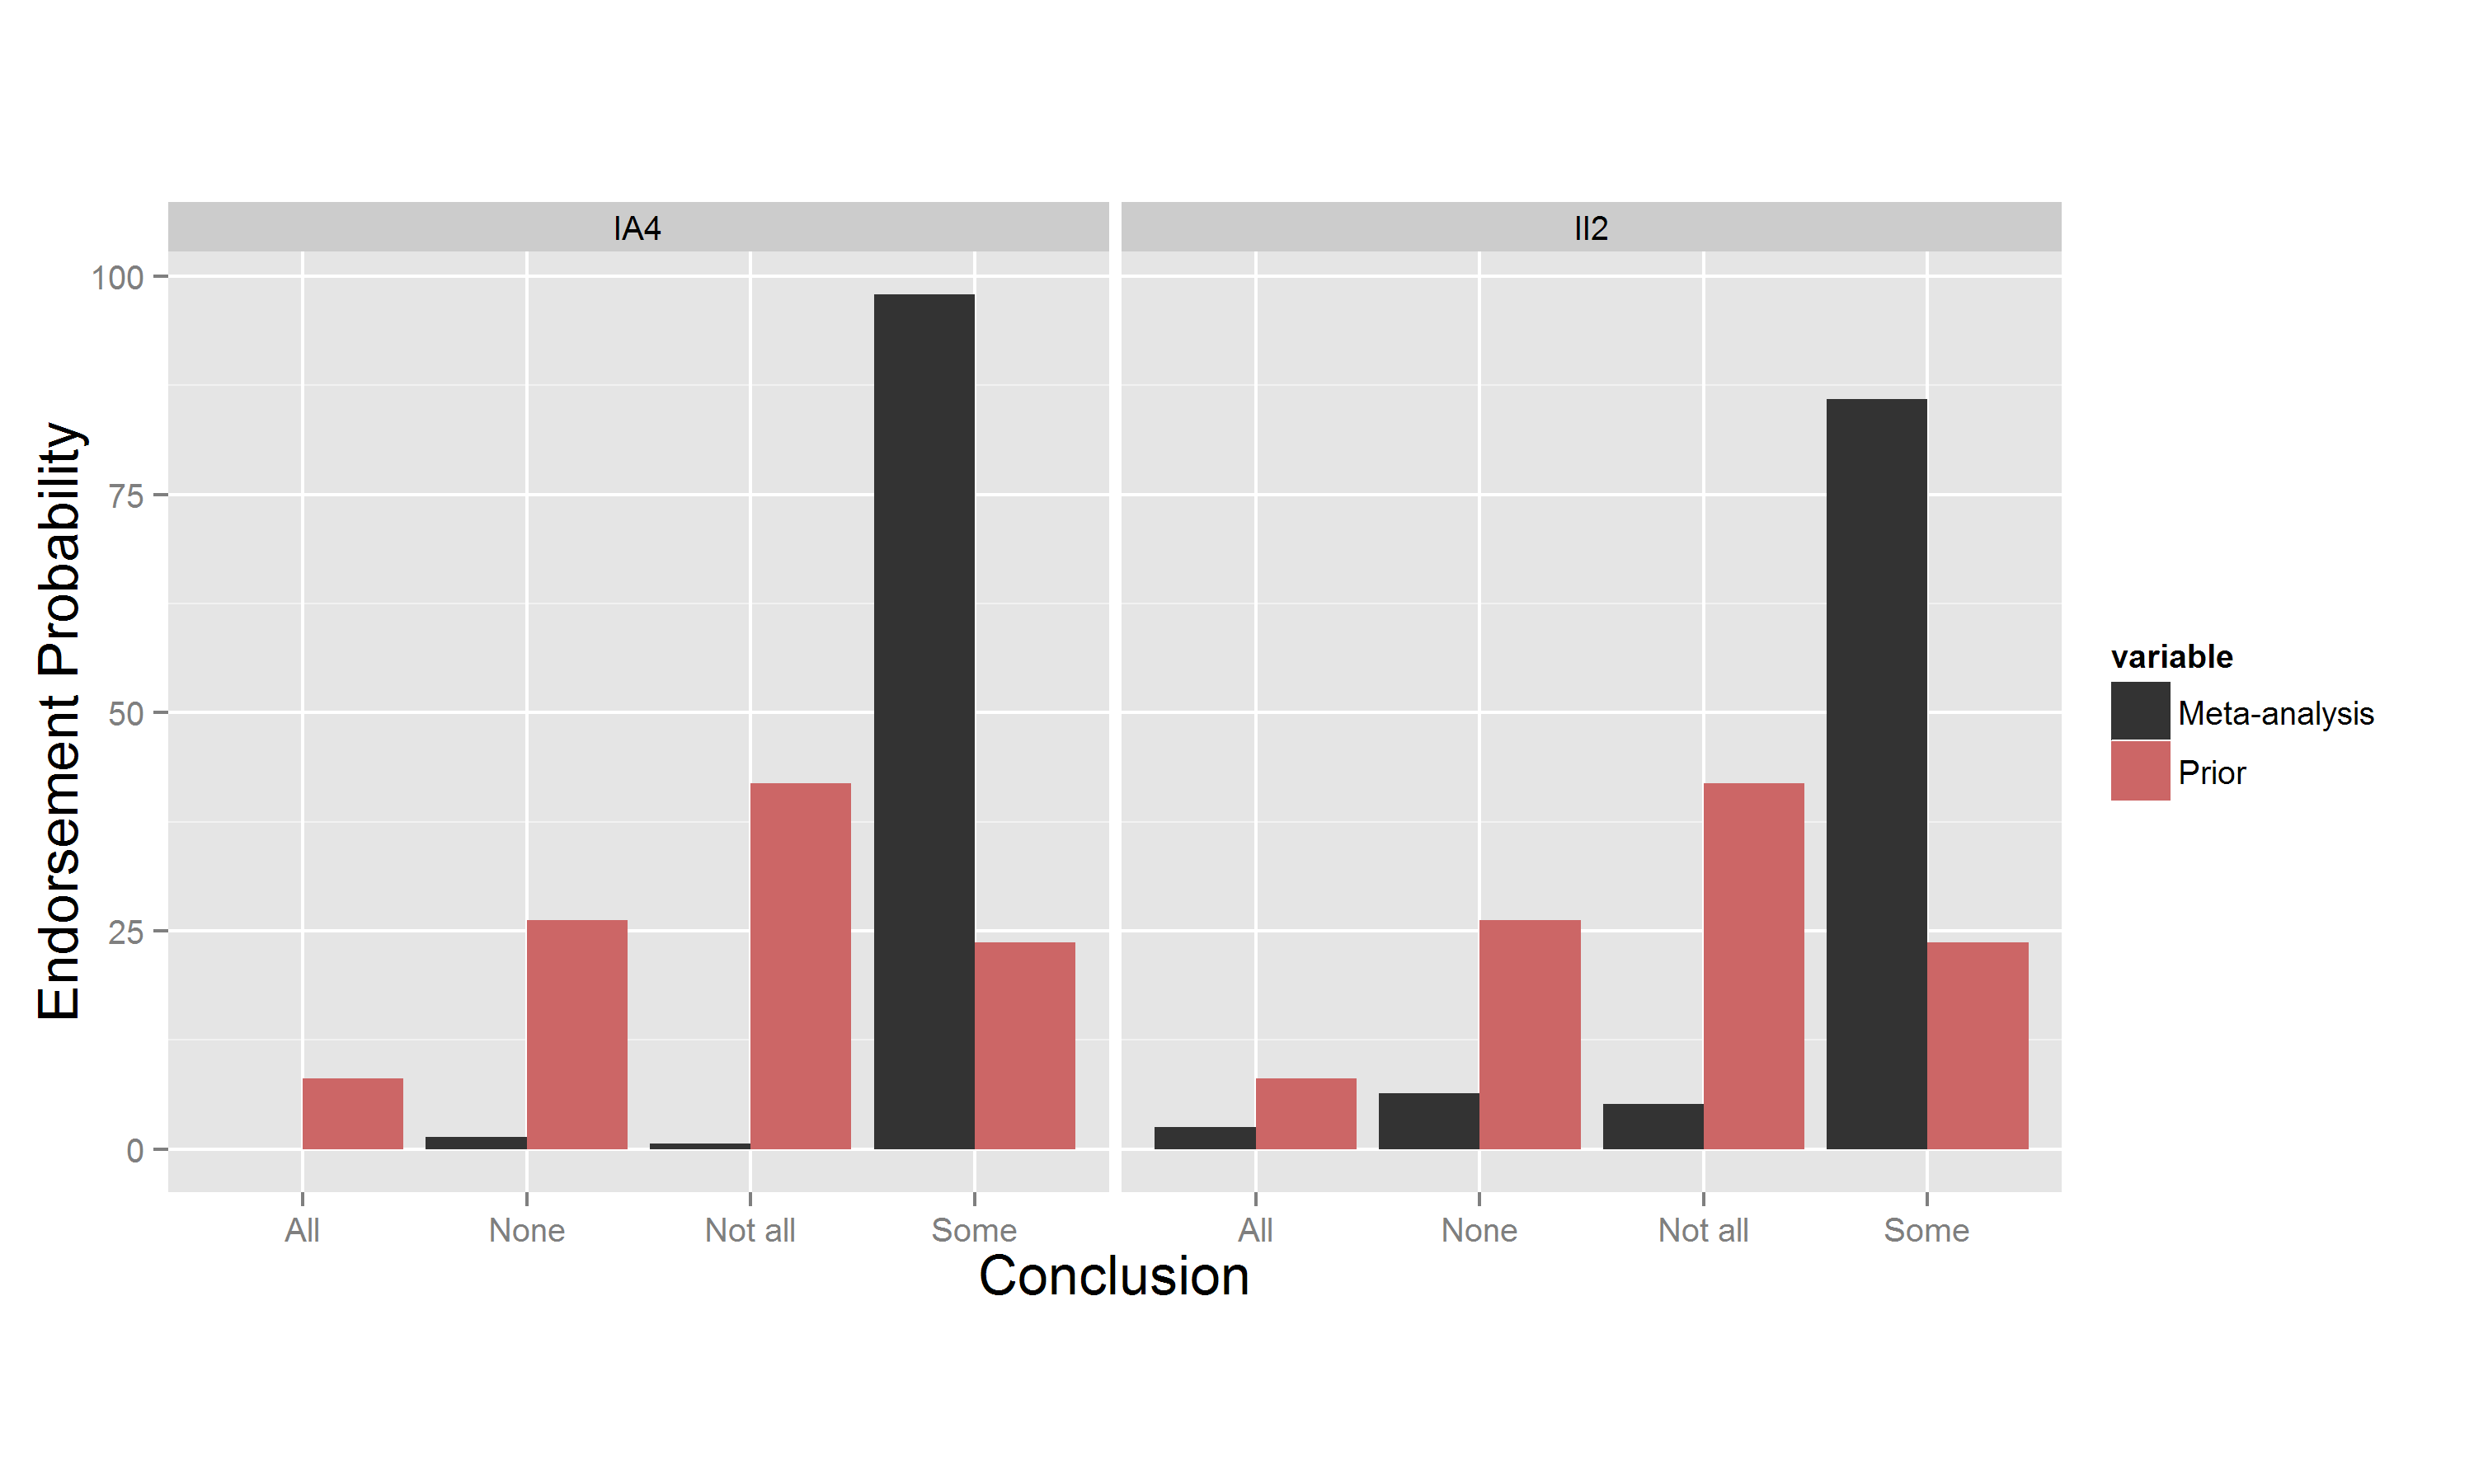
\includegraphics[width = {0.66\columnwidth}]{multibar_alpha1_prior}
%	\label{fig:subfigure1}}
%%\caption{Single-model, valid}}
%%\hfill
%\subfigure[conditional semantics]{ %}
%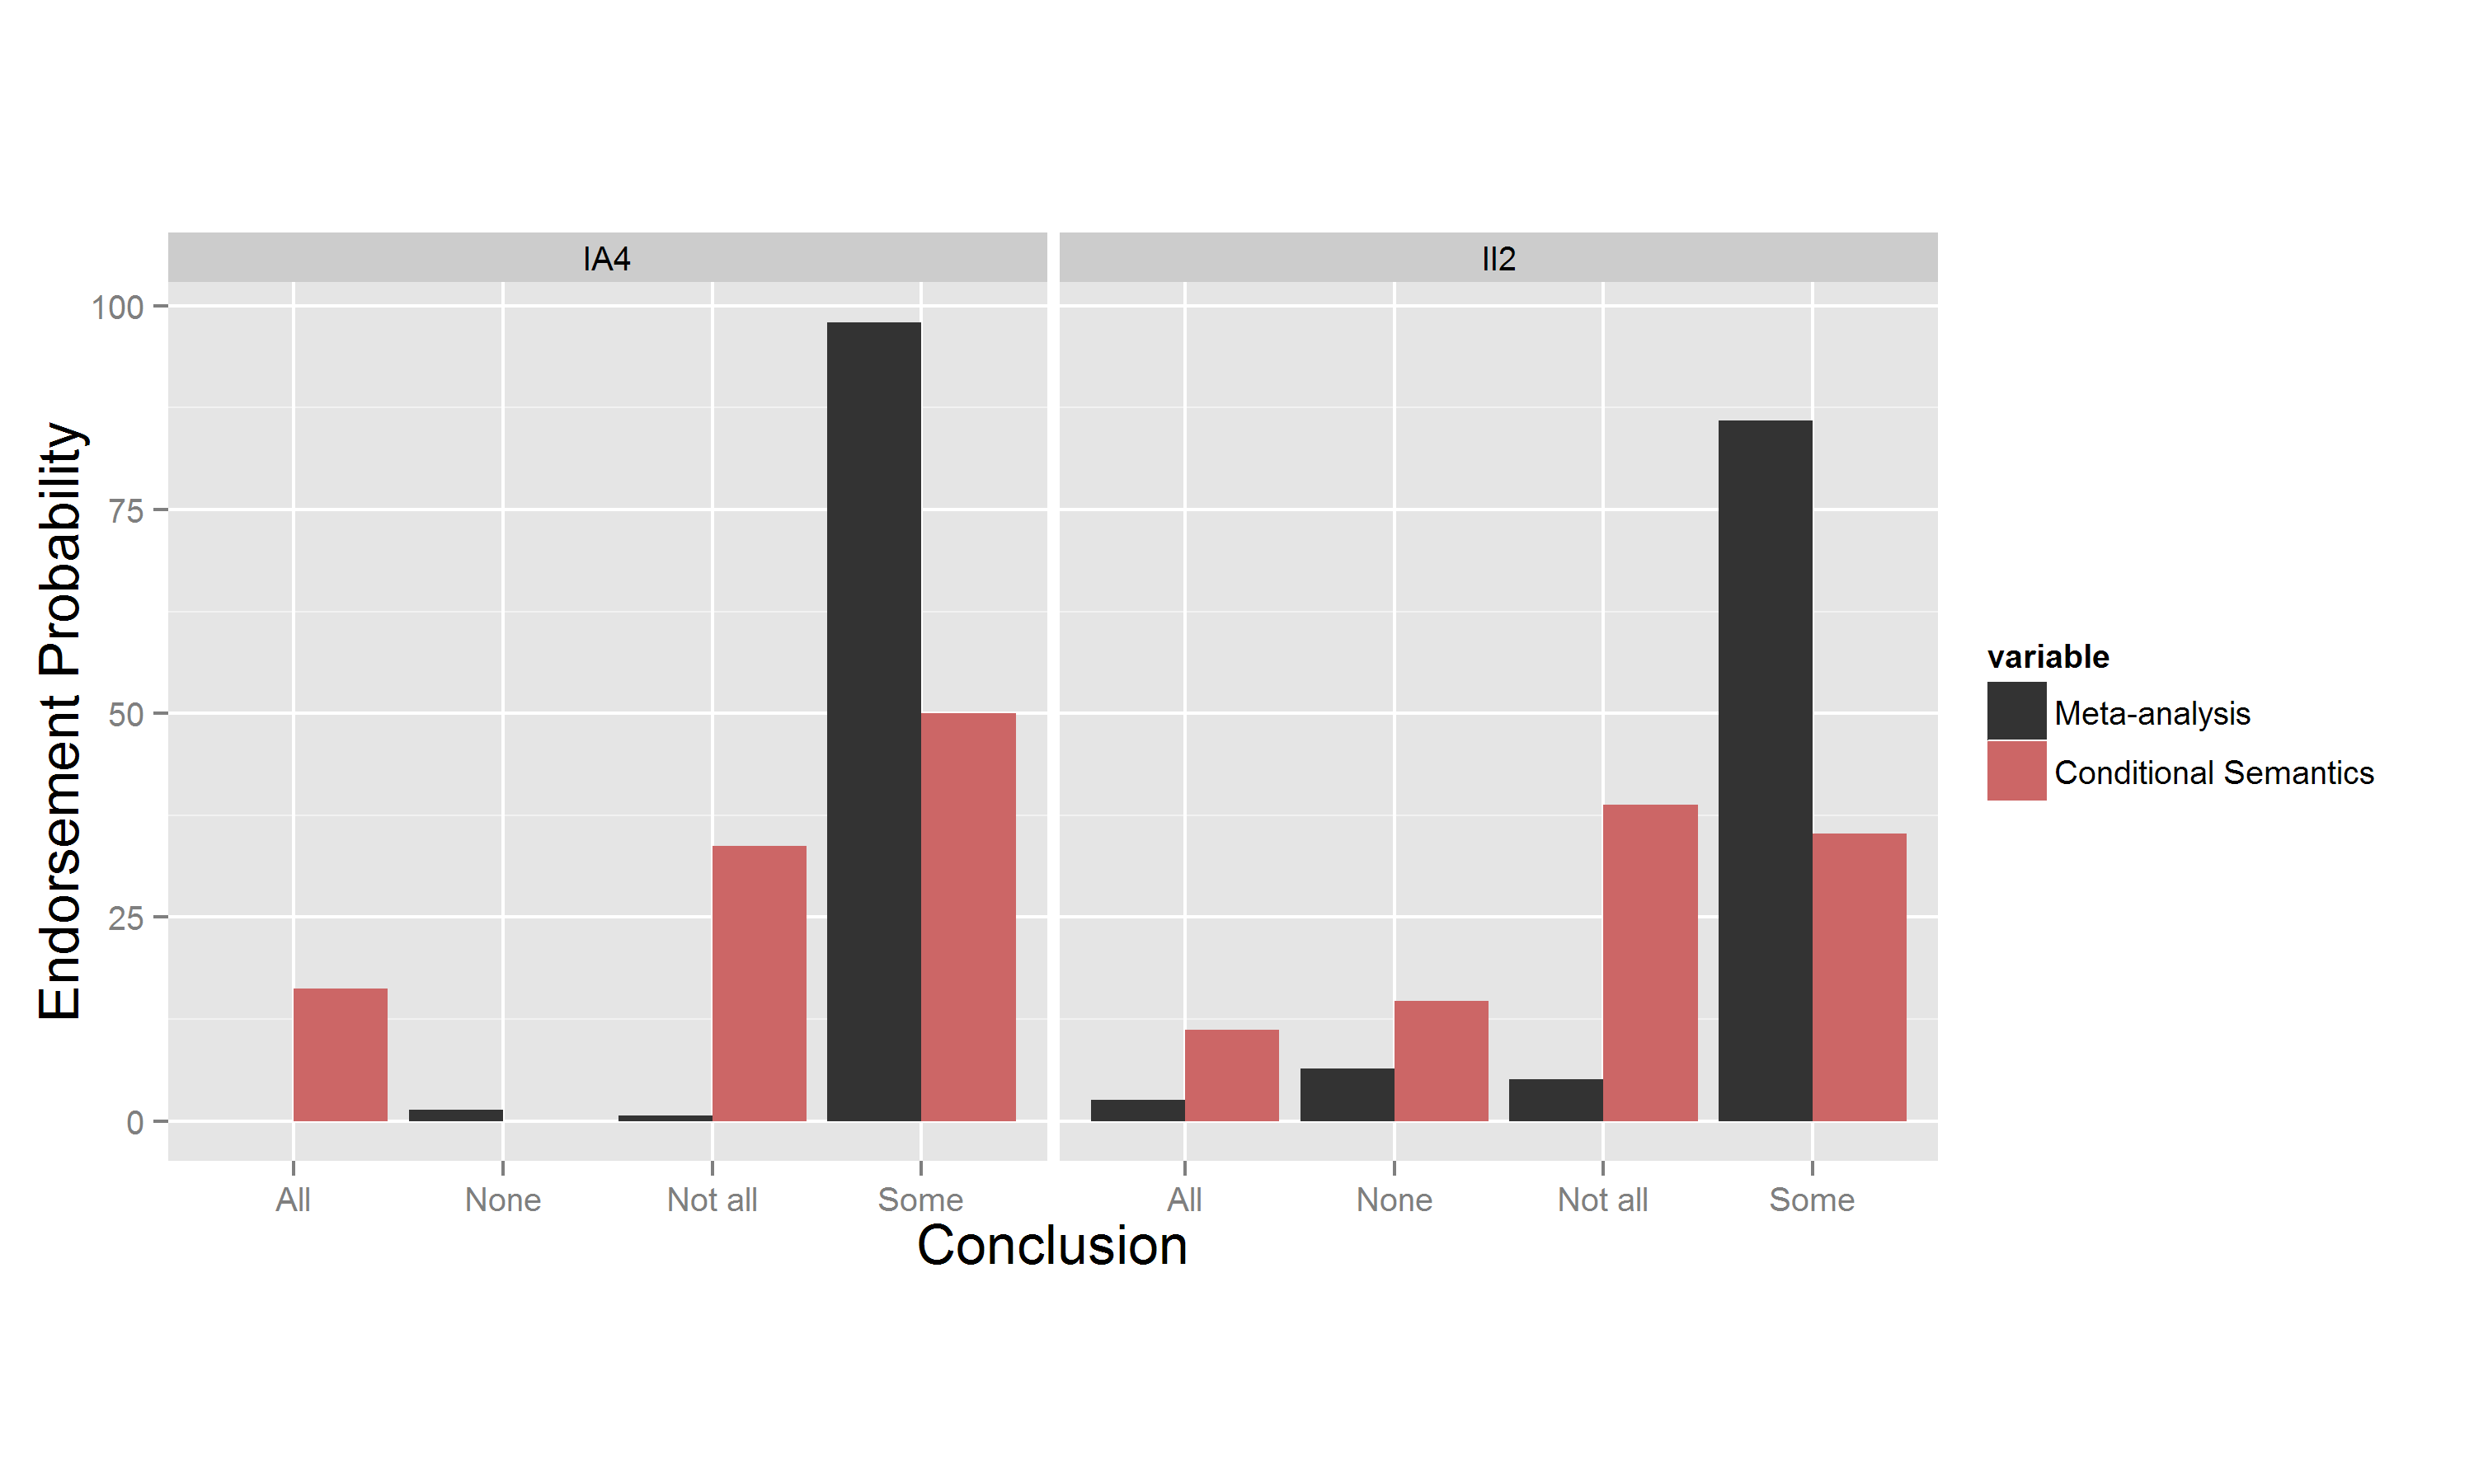
\includegraphics[width = {0.66\columnwidth}]{multibar_alpha1_lit}
%%\label{fig:subfigure3}
%\caption{Multiple-model, valid}
%}
%%\hfill
%\subfigure[conditional pragmatics]{
%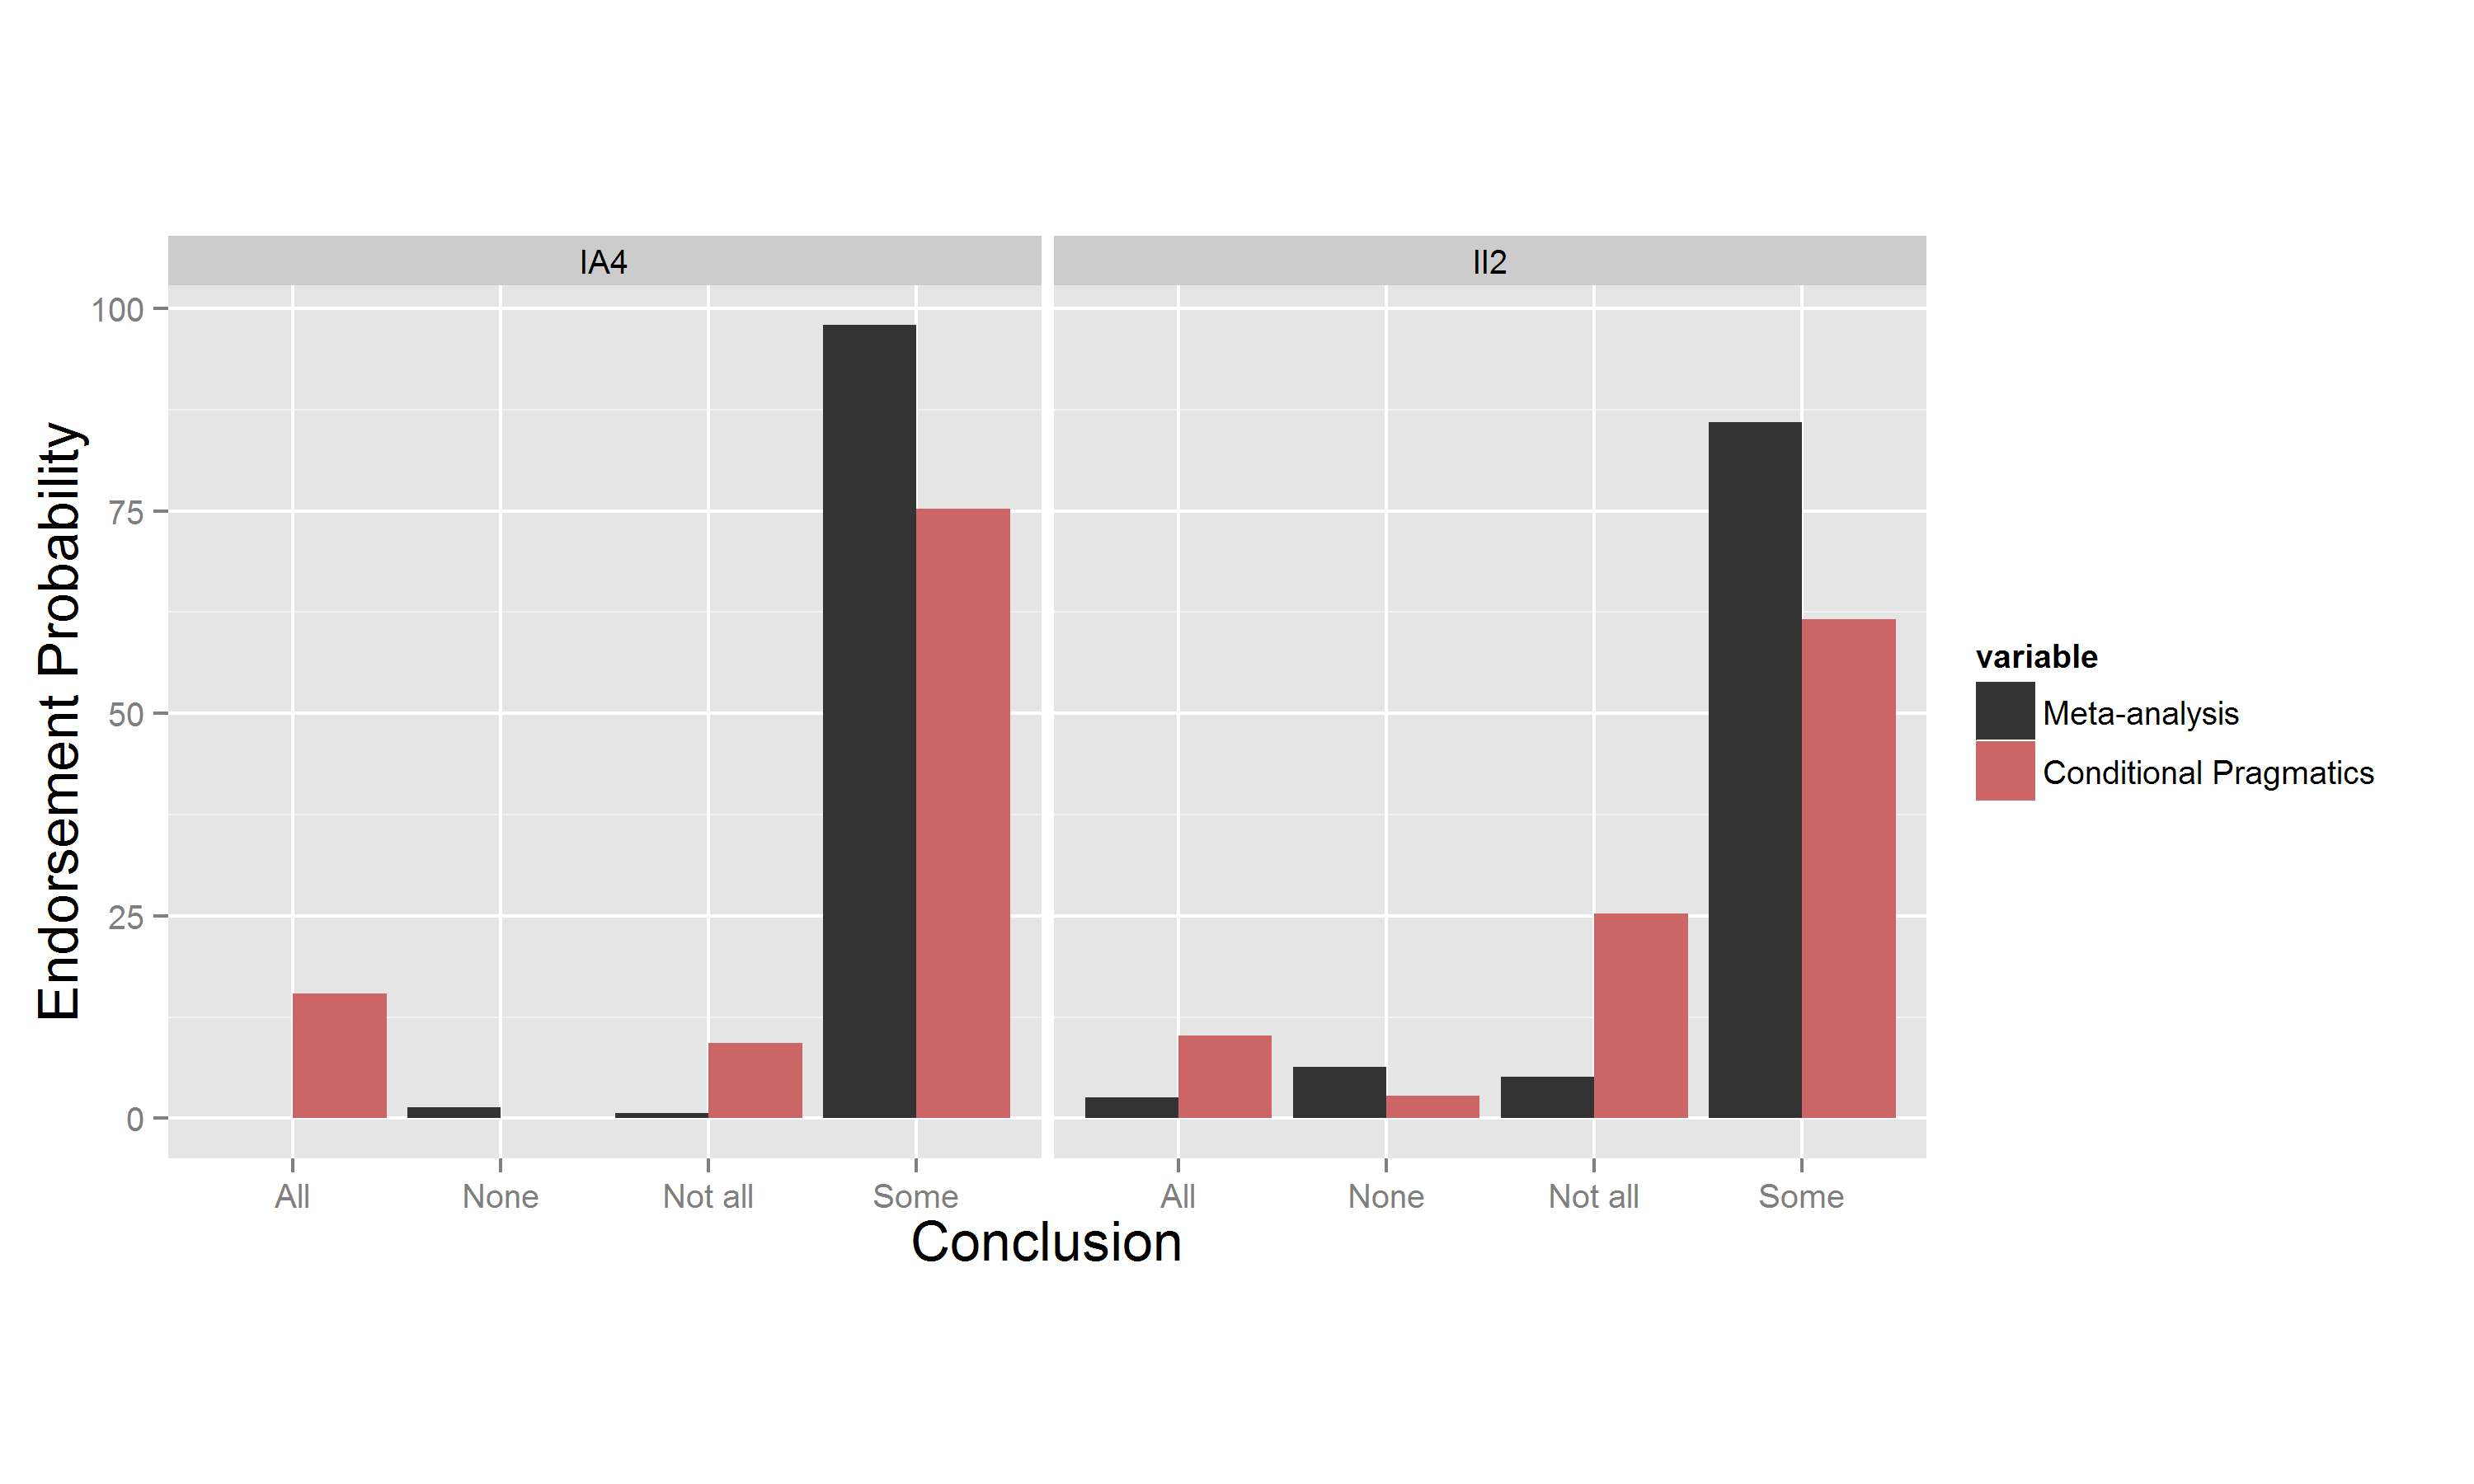
\includegraphics[width = {0.66\columnwidth}]{multibar_alpha1_prag}
%%\label{fig:subfigure5}
%\caption{invalid}
%%}
%%\quad
%%
%%\subfigure[one model, valid]{ %
%%\includegraphics[width = {0.66\columnwidth}]{IA4_boxplot_text}
%%%\label{fig:subfigure2}}
%%\hfill
%%\subfigure[multiple models, valid]{
%%\includegraphics[width = {0.66\columnwidth}]{EI3_boxplot_text}
%%%\label{fig:subfigure4}}
%%\caption{Multiple-model, valid}
%%\hfill
%%\subfigure[invalid]{
%%\includegraphics[width = {0.66\columnwidth}]{AA2_boxplot_text}
%%%\label{fig:subfigure6}}
%%\caption{invalid}
%%
%%\caption{Participants' endorsements in six syllogisms}
%%\label{fig:fig1}


%
%
%Mental Models Theory explains difficulty in syllogisms by demonstrating that multiple, distinct situations can be consistent with a pair of premises, giving rise to different possible conclusions. Valid syllogistic conclusions arise in every possible model. (This is the same notion of Pr(conclusion | premises) = 1). 
%
%This is always the case the logically invalid syllogisms (see discussion below), and is sometimes the case with logically valid syllogisms.

%\subsubsection{Logical invalidity}
%For syllogisms that have no valid conclusion, the probabilistic reasoner computes the probability of the conclusion conditioned on the premises being true by sampling. For all invalid syllogisms, this yield a gradeds response across the different possible conclusion types. 
%
%
%\subsubsection{Logical validity}
%A conclusion is logically valid if and if only it is true in all possible situations. Recall that possible situations are restricted to those that are consistent with the premises. The universal quantifiers (all, none) entail their particular counterparts (some, not-all), respectively. This was noticed by Aristotle and commonly visualized in the \emph{Square of Opposition}. For our probabilistic reasoner, confidence for {\emph all} and {\emph some} (to take the affirmative case) will be both maximal. {\emph All} is always true and {\emph some} is true whenever {\emph all} is true.





\section{Most and few}

Since our model is based on a truth-functional semantics, it is able to deal with any quantified sentence, so long as the quantifier can be mapped to a truth-functional operator. The question of the meaning of generalized quantifiers like ``most" and ``few" is of great interest to the field of formal semantics. Often, ``most" and ``few" are modeled by a thresholded step function. As a first test of the generality of the model, we define most and few by a threshold of 0.5. 

We compare our model predictions to a study carried out by Chater \& Oaksford on syllogisms using these generalized quantifiers. 

\section{Discussion}

We have presented a formal model of syllogistic reasoning based on the rational speech-act framework. We have shown that in this model, reasoners construct mental situations by sampling, and reason over these situations, much like has been described in the Mental Models literature. Unlike Mental Models, however, our model is inherently probabilistic and thus assumes reasoners are in some way gaging degrees of plausibility when it comes this sort of logic task. Further, this model is fundamentally quantitative, and thus elaborates on the Mental Models theory in a novel way.

In this framework, a syllogism is read as an argument given as a part of discourse between people. Indeed, this is how syllogisms were used in the time of Aristotle and in the long tradition of scholastic philosophers. Fundamentally, they are a tool used to convince others. The results of the pragmatic reasoning model shed light on the idea that human reasoning behavior in the syllogistic task is as much reason as it is human. Gaging degrees of plausibility alone is not sufficient. A listener needs to be posited at the end of the line so that a conclusion makes sense; so that a conclusion is convincing!

If one accepts that the purpose of a syllogism is to convince, a natural question arises. Why not just assert ``Socrates is mortal" from the start? Why go through the trouble of laying out premises and have a person draw the conclusion? Arguments are used to persuade, and not all assertions are equally believable a priori. The reason premises are presented is that some of us may believe Socrates is actually not mortal; after all, we're still talking about him 2400 years after he lived. And so the conclusion is not obvious, and the premises are an alternative route to persuasion. If we accept the premises, we are left with no choice but to draw the conclusion.

We set out to test this intuition by seeing if the middle term had special significance. The rationale is that if someone is to go through the trouble of mentioning the middle term, it must allow them to assert something that they wouldn't be able to assert otherwise. In other words, we take the a priori probability of A \& C to be relatively low, but become higher if B is observed. A \& C become correlated via B. This is akin to saying that the end terms have a special relationship via the middle term. It is no coincidence that the same middle term appears in both premises and it is no coincidence the premises appear at all. 

We modified the naive binomial prior to induce a slight correlation between A \& C via B. Overall, the model gets a few more questions correct and provides a better quantitative fit to the data. We also looked at its effects in the generalized quantifier model and the effect is I HOPE THE EFFECT IS GOOD. 

\bibliographystyle{apacite}

\setlength{\bibleftmargin}{.125in}`
\setlength{\bibindent}{-\bibleftmargin}

\bibliography{mhtbib}


\end{document}